\documentclass[avery5371,grid,frame]{flashcards}

\usepackage[pdftex]{graphicx}
\usepackage{multicol}
\cardfrontstyle[\large\slshape]{headings}
\cardbackstyle{empty}



\begin{document}

\cardfrontfoot{3AUA}

\begin{flashcard}[Gand VGS]{Måleblende\\Fordeler/Ulemper}
	\begin{multicols}{2}
		\begin{description}
			\item [Fordeler]
			\item Enkel å produsere
			\item fås i alle dimensjoner
			\item høye trykk og temperaturer
		\columnbreak
			\item [Ulemper]
			\item  Ulineært målesignal $\sqrt{\Delta P}$ 
			\item  groing reduserer målenøyaktighet 
		\end{description}
	\end{multicols}
\end{flashcard}

\begin{flashcard}[Gand VGS]{Turbinmåler\\Fordeler/Ulemper}
	\begin{multicols}{2}
		\begin{description}
			\item [Fordeler]
			\item Svært nøyaktig med rette forhold
		\columnbreak
			\item [Ulemper]
			\item Følsom for endring i viskositet
			\item Følsom for endring i massetetthet
		\end{description}
	\end{multicols}
\end{flashcard}

\begin{flashcard}[Gand VGS]{Elektromagnetisk Flowmåler\\Fordeler/Ulemper}
	\begin{multicols}{2}
		\begin{description}
			\item [Fordeler]
			\item god målenøyaktighet
			\item ikke trykktap
			\item ingen beveglige deler
			\item takler slipende og korrosive partikler
			\item måler begge retninger
			\item nøyaktighet påvirkes lite av \\ viskositet og massetetthet
		\columnbreak
			\item [Ulemper]
			\item må ledende væske
		\end{description}
	\end{multicols}
\end{flashcard}

\begin{flashcard}[Gand VGS]{Vortexmåler\\Fordeler/Ulemper}
	\begin{multicols}{2}
		\begin{description}
			\item [Fordeler]
			\item ingen beveglige deler
			\item langtidsstabil
			\item nøyaktighet påvirkes lite av \\massetetthet
		\columnbreak
			\item [Ulemper]
			\item skaper trykkfall
			\item følsom for vibrasjoner
			\item lav hastighet kan gi målefeil
			\item krever laminær strømning
			\item 
		\end{description}
	\end{multicols}
\end{flashcard}


\begin{flashcard}[Gand VGS]{Coriolis-måler\\Fordeler/Ulemper}
	\begin{multicols}{2}
		\begin{description}
			\item [Fordeler]
			\item enkel mekanisk konstruksjon
			\item god målenøyaktighet
			\item takler pulserende strømning
			\item ufølsom for endring i:\\trykk,viskositet og massetetthet
			\item takler gassbobler og partikler
			\item mulig med avlesning av temperatur, \\ viskositet og massetetthet
		\columnbreak
			\item [Ulemper]
			\item dyr??
		\end{description}
	\end{multicols}
\end{flashcard}

\begin{flashcard}[Gand VGS]{Ultralyd flowmåler\\Fordeler/Ulemper}
	\begin{multicols}{2}
		\begin{description}
			\item [Fordeler]
			\item Ingeni restriksjon i røret
			\item enklere å montere for versjoner med sensor utenpå røret
			\item finnet i versjoner med høy nøyaktiget
		\columnbreak
			\item [Ulemper]
			\item følsomme for gassbobler og partikler ved væskemåling
			\item må kompensere for trykk og temperatur veg gassmåling
			\item kan gi stor feilmåling dersom røret ikke er fult av væske
		\end{description}
	\end{multicols}
\end{flashcard}

\begin{flashcard}[Gand VGS]{2-leder kobet strømsløyfe}

$\includegraphics[height=4cm]{../book/current11.eps}$
\end{flashcard}

\begin{flashcard}[Gand VGS]{Formel for strømning i flowmeter \\ med differansetrykk}

  \begin{description}
    \item [Variabel massetetthet] $Q = k \sqrt{{P_1 - P_2} \over \rho}$ 
    \item [Konstant massetetthet] $Q = k \sqrt{P_1 - P_2 }$ 
  \end{description}


\end{flashcard}

\begin{flashcard}[Gand VGS]{Måleblende}
	\begin{minipage}{0.35\textwidth}
	Flow: $Q = k \sqrt{{P_1 - P_2} \over \rho}$ 
	\\
	Kvadratrotuttrekker gjør målinger i nedre del av range unøyaktige
	\end{minipage}
	\begin{minipage}{0.65\textwidth}
$\includegraphics[width=1\textwidth]{../book/inverse_023.eps}$
	\end{minipage}


\end{flashcard}

\end{document}
